\subsection{Information Theory}
Information theory is the mathematical study of the quantification, storage, and communication of information. By Claude Shannon. 
A key measure in information theory is \emph{entropy}. Entropy quantifies the amount of uncertainty involved in the value of a random variable or the outcome of a random process.
For example, identifying the outcome of a fair coin flip (which has two equally likely outcomes) provides less information (lower entropy, less uncertainty) than identifying the outcome from a roll of a die (which has six equally likely outcomes).


\subsection{Security Definitions}
\begin{defn}
    Computationally Secure: it takes N operations using the \textbf{best known algorithm} to break a crytographic system and N is too large to be feasible.
\end{defn}

\begin{defn}
    Provably Secure: breaking the system is reduced to solving some well-studied hard problem.
\end{defn}

\begin{defn}
    Unconditional Secure/Perfectly Secure: the system is secure against an adversary with unlimited computational power.
\end{defn}

Key size is important. Advances in computer hardware and algorithms are important. In the future, it will be broken due to hardware or better algorithms.

\subsection{Probability and Ciphers}

\begin{defn}
Let $P$ denote the set of plaintexts, $K$ the set of keys, and $C$ denote the set of cipher texts. $p(P=m)$ is the probability that the plaintext is $m$. Then,
\[
p(C=c) = \sum_{k: c\in \mathbb{C}(k)} p(K=k)\cdot p(P=d_k(c))
\]
\end{defn}

This formula calculates the probability of a specific cipher text $C = c$ occuring. It sums over all keys $k$ that could result in the ciphertext $c$ , combining the probabilities of the key and the corresponding plaintext. It is fundamental in several cryptographic analyses:
\begin{itemize}
    \item Ciphertext distribution: compute the distribution of the ciphertexts given the plaintext and key distributions. By ensuring $p(C=c)$ is uniform, cryptographers achieve perfect secrecy in schemes like the One-Time Pad.
    \item Evaluating security metrics: the uncertainty of $C$ is maximized for a secure cipher, ensuring that an attacker cannot infer patterns.
\end{itemize}



\subsection{Perfect Secrecy}
Previously, the ciphertext revelas a lot of information about the plaintext. We want a system in which ciphertext does not reveal anything about the plaintext. 

\begin{defn}
    Perfect secrecy: a cryptosystem has perfect secrecy if \[ p(P=m | C=c) = p(P=m) \] for all plain texts $m$ and ciphertexts $c$.
\end{defn}

\begin{lem}
    Assume the cryptosystem is perfectly secure, then 
    \[ \#K \geq \#C \geq \#P\] where $\#$ denotes the number of items in the corresponding set. 
\end{lem}

\subsubsection{One-Time Pad}

\begin{thm}
    Shannon's Theorem: Let $(P, C, K, e_k(), d_k())$ denote a cryptosystem with \( \#K = \#C = \#P\). Then the cryptosystem provides \emph{perfect secrecy} if and only if:
    \begin{itemize}
        \item Every key is used with equal probability $1/\#K$
        \item For each $m \in P$ and $c \in C$, there is a unique key $k$ such that $c = e_k(m)$
    \end{itemize}
\end{thm}

\begin{defn}
One-Time Pad a cryptographic system that provides perfect secrecy when implemented correctly. It is a symmetric encryption technique (shift cipher) where the sender and receiver use a shared secret key, known as the pad, that is as long as the plaintext message. 
\[\#K = \#P = \#C = 26^n\]
and $p(K=k) = 1/26^n$. Also known as the Vernam cipher. It is perfectly secure because:
\begin{itemize}
    \item The key is truly random
    \item The key is as along as the plaintext
    \item The ciphertext reveals no information about the plaintext. The ciphertext $C$ is independent of the plaintext $P$ without the key $K$, and observing the ciphertext does not reduce the uncertainty about the plaintext.
    \item The key is used only once (hence the name)
\end{itemize}
\end{defn}

\textbf{Example:} Suppose the plaintext \( P \) is "A", and the key \( K \) is a random letter. After encryption, the ciphertext \( C \) could be any letter, with equal probability. If an attacker intercepts \( C = Z \), they cannot determine whether the plaintext \( P \) was "A", "B", or any other letter without the key. Every possible plaintext is equally likely.

\subsection{Entropy}
Due to the key distribution problem (the key must be as long as the message), perfect secrecy is not practical. Instead, we need a cryptosystem in which \textbf{one key can be used many times}, and \textbf{a  small key can encrypt a long message}. Such a system is not perfectly secure, but it should be computationally secure. We need to measure the amount of information first: Shannon's entropy. \\

\begin{defn}
    Shannon's Entropy: Let $X$ be a random variable which takes a finite set of values $x_i$, with $1 \leq 1 \leq n$, and has a probability distribution $p(x)$. We use the convention that if $p_i = 0$ then $p_i \log_2(p_i) = 0$. The entropy of $X$ is defined as:

    \[ H(X) = -\sum_{i=1}^n p_i \cdot \log_2 p_i\] 

    Properties:
    \begin{itemize}
        \item $H(X) \geq 0$
        \item $H(X) = 0$ if $p_i = 1$ and $p_j = 0$ for $i \neq j$
        \item if $p_i = 1/n$ for all $i$, then $H(X) = \log_2(n)$
    \end{itemize}
\end{defn}

\textbf{Example:} For a specific question X: ``Will you go out with me?'', the answer is Yes or No. If you always say No, the amount of information, $H(X) = 0$. If you always say Yes, $H(X) = 0$. You know the result. If you say Yes and No with equal probability, $H(X) = 1$. When you get the answer, no matter what it is, you learn a lot. Here, $H()$ is the entropy, and is independent of the length of $X$.

\subsection{Joint Entropy, Conditional Entropy and Mutual Information}
Used to measure the uncertainty and interdependence between random variables. 

\begin{defn}
    The \textbf{joint entropy} of two random variables $X$ and $Y$ measures the total uncertainty in the pair $(X,Y$), considering them together. The total amount of information contained in \emph{one} observation of both $X$ and $Y$. 
    \[
H(X, Y) = -\sum_{x \in X} \sum_{y \in Y} P(x, y) \log_2 P(x, y)
\]

where $P(x,y)$ is the joint \emph{probability} of $X=x$ and $Y=y$.

\[H(X,Y) \leq H(X) + (HY) \]
\end{defn}

\begin{defn}
The \textbf{conditional entropy} of $X$ given $Y$, $H(X|Y)$, measures uncertainty in $X$ after knowing $Y$. It quantifies how much information about $X$ is still unknown once $Y$ is known.

The entropy of $X$ given an observation of $Y=y$:
\[H(X \mid Y = y) = -\sum_{x} p(X = x \mid Y = y) \cdot \log_2 p(X = x \mid Y = y).
\]

Then,
\[H(M \mid C) = \sum_{c} p(C = c) \cdot H(M \mid C = c) 
= - \sum_{m} \sum_{c} p(C = c) \cdot p(M = m \mid C = c) \cdot \log_2 p(M = m \mid C = c). \]    
\end{defn}

\begin{defn}
    Conditional and joint entropy are connected as follows:
    \[H(X,Y) = H(Y) + H(X|Y) \]
    \[ H(X|Y) \leq H(X)\]
\end{defn}

\begin{defn}
\textbf{Mutual information} quantifies the amount of shared information between $X$ and $Y$. It measures how much knowing $X$ reduces the uncertainty about $Y$ (or vice versa). The expected amount of information that $Y$ gives about $X$ (or $X$ about $Y$).

\[
I(X; Y) = H(X) + H(Y) - H(X, Y) =  H(Y) - H(Y \mid X) = H(X) - H(X \mid Y)
\]

Mutual information represents the reduction in uncertainty about one variable due to knowledge of the other. If $X$ and $Y$ are independent, $I(X; Y)$ because knowing one provides no information about the other.
\end{defn}

\textbf{Example}
Suppose \( X \) and \( Y \) represent the outcomes of rolling two six-sided dice:
\begin{itemize}
    \item \( H(X) \): Entropy of die \( X \) (e.g., how random die \( X \)'s outcomes are).
    \item \( H(X, Y) \): Joint entropy, the uncertainty of the combined outcome of \( X \) and \( Y \).
    \item \( H(Y \mid X) \): Given a roll of \( X \), the remaining uncertainty in \( Y \).
    \item \( I(X; Y) \): Shared information (likely 0 if the dice rolls are independent).
\end{itemize}

\begin{figure}[h!]
    \centering
    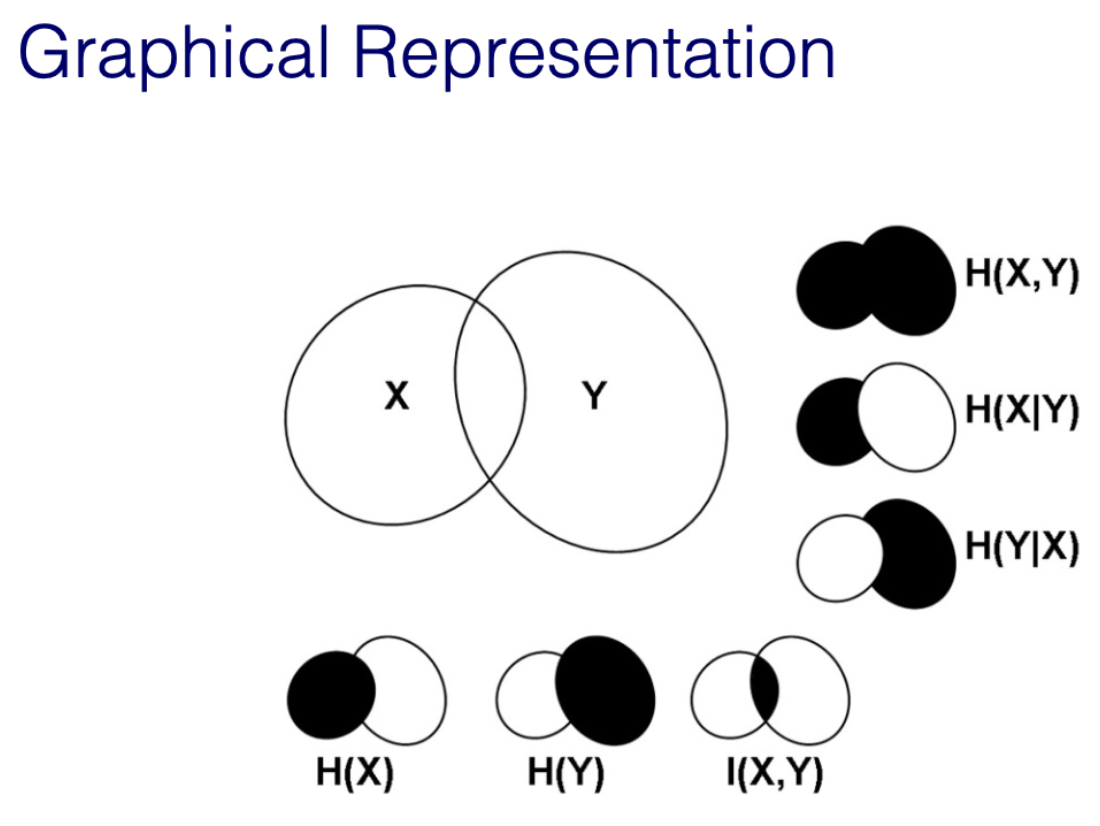
\includegraphics[scale=0.4]{img/entropy.png}
\end{figure}

\subsubsection{Application to Ciphers}
\begin{itemize}
    \item $H(P|K,C) = 0$: If you have the cipher text and the key, you can decrypt and obtain the plaintext. There is no surprise, hence 0.
    \item $H(C|P,K) = 0$: When you have the key and the plaintext to can encrypt and obtain the ciphertext. True for deterministic cryptosystems. Not for modern ones that use randomness (the same plaintext can be encrypted with the same key but correspond to a different ciphertext).
    \item $H(K,C) = H(K) + H(P)$
    \item Then, $H(K|C) = H(K,C) - H(C) = H(K)+H(P)-H(C)$. Given the ciphertext, can we obtain information of the key?
\end{itemize}

\subsection{Spurious Keys and Unicity Distance}

\begin{defn}
    Spurious keys: the remaining possible but incorrect keys.
\end{defn}

Tactic of an attacker is to reduce the number of spurious keys to zero. Then the one correct key remains.

Plaintext are not random: natural languages... Random text has an entropy of $H_L = 4.7$ bits (5 bits per letter).
\Comment{continue...}

\subsubsection{Entropy of a Natural Language}
\begin{defn}
    The entropy of a natural language measures the average \emph{amount of information} conveyed per character, word, or sentence in that language, accounting for redundancy and patterns in its structure. It is defined by 
    \[H_L = \lim_{n\rightarrow\infty}\frac{H(P^n)}{n}\]
    where $n$ is the length of letters, and $P^n$ is the n-grams.
\end{defn}

For English (estimation): $1.0 \leq H_L \leq 1.5$ bits per character. This means you need 5 bits of data to represent only 1.5 bits of information. Natural languages are highly redundant (e.g., letter and word patterns), making them less random than completely independent symbols.
The low entropy of natural languages makes cryptographic attacks easier because it introduces predictability and redundancy (useless information) in the plaintext, which attackers can exploit. To mitigate this, cryptographic systems should:
\begin{itemize}
    \item Use strong encryption methods that destroy plaintext patterns (e.g., AES or OTP).
    \item Introduce randomness (e.g., padding).
    \item Avoid predictable plaintext in sensitive communications.
\end{itemize}

\subsubsection{Redundancy}
\begin{defn}
    Redundancy is information that is expressed more than once. The repetition or predictability of information, where certain elements (like letters, words, or phrases) appear more frequently or follow patterns. It is defined as:
    \[ R_L = 1-\frac{H_L}{\log_2 \#\mathbb{P}
    }\]

    where $\#\mathbb{P}$ is the message space.
\end{defn}

\textbf{Example}: For English,
\[R_L \approx 1-\frac{1.25}{\log_2 26} = 0.75 \]
This means 75 percent redundancy, 75 \% of the information in a message is predictable or can be removed without losing meaning. You can zip your files 3 quarters. 

\begin{defn}
    The \textbf{average number of spurious keys} is:
    \[\bar{s}_n \geq \frac{\#\mathbb{K}}{ \#\mathbb{P}^{n\cdot R_L}}-1 \]
    An attacker wants this number to be zero.
\end{defn}

We can make this number zero making the number of keys equal to the number of n-grams times the redundancy. This leads to unicity distance.

\subsubsection{Unicity Distance and Ciphers}
\begin{defn}
    \textbf{Unicity distance} is the average number of cipher texts for which the expected number of spurious keys becomes 0. 
    \[ n_0 \approx \frac{\log_2 \#\mathbb{K}}{R_L \cdot \log_2 \#\mathbb{P}}\]
\end{defn}

In the context of a substition cipher, the unicity distance is the length of the ciphertext required for an attacker to break the cipher with high probability (i.e., to uniquely determine the key). It depends on the number of possible keys and the redundancy of the language used.
Given $\#P=26, \#K=26!, R_L =0.75$, 
\[n_0 \approx \frac{88.4}{0.75 \cdot 4.7} \approx 25\]
To successfully break the cipher (i.e., determine the correct key), an attacker needs to analyze at least 25 characters of ciphertext. This is because, with this many characters, the redundancy and patterns in the language (due to its predictable letter frequencies) will provide enough information for the attacker to determine the key. This highlights the cipher's vulnerability: there are $26!$ possible keys! The smaller the unicity distance, the easier it is to break the cipher with limited ciphertext. \\

For a modern stream cipher $\#P=2$ (binary symbol 0 or 1), $\#K=2^l, R_L =0.75$, then 
\[ n_0 \approx \frac{l}{0.75} = \frac{4\cdot l}{3}\] 

Here, the unicity distance tells us how many ciphertext bits are needed to break the streamcipher. The distance is proportional to the key length $l$. Longer key lengths lead to larger unicity distances, making it harder to break the cipher. \\

With no redundancy, $R_L = 0$. Then:
\[ n_0 \approx \frac{l}{0} = \infty \]

There are no predictable patterns in the plaintext. Perfect randomness would imply that every symbol in the plaintext carries the maximum amount of information, with no repeated or predictable patterns.In such a case, the language would have maximum entropy, and there would be no chance of making guesses about the plaintext from patterns in the ciphertext. In practice: no natural language has zero redundancy.